% ============================================================================
% sections/sec5_results.tex
% ============================================================================
\section{Results and Discussion}
\label{sec:results}

All figures below are drawn directly from \texttt{results/path\allowbreak\_a\allowbreak\_report.md},
generated by \ringcode{run\allowbreak\_full\allowbreak\_evaluation.py} across the eight independent
seeds described in \Cref{sec:multiseed}: 200 queries per seed, 1{,}600 queries
per system in total, mean $\pm$ 95\% confidence interval (Student's-$t$)
throughout. The single-seed sanity check in \ringcode{run\allowbreak\_omniguard\allowbreak\_benchmark.py}
was re-run immediately before writing this section and reproduces the same
qualitative picture at $n{=}200$, single seed.

\subsection{Main System Comparison}

\Cref{tab:main-comparison} and \Cref{fig:main-comparison} compare all six
systems across all six attack regimes described in \Cref{sec:attack-simulator}.

\begin{table}[htbp]
\centering
\small
\resizebox{\textwidth}{!}{%
\begin{tabularx}{1.12\textwidth}{@{}l Y Y Y Y Y Y@{}}
\toprule
\textbf{Defense Framework} & \textbf{Accuracy} & \textbf{Overall ASR} & \textbf{PIDP ASR} & \textbf{Collusion ASR} & \textbf{Stealth ASR} & \textbf{Silent ASR} \\
\midrule
Vanilla RAG            & \pmci{85.1}{0.1} & \pmci{0.9}{0.2} & \pmci{1.2}{0.6} & \pmci{1.5}{0.4}  & \pmci{1.1}{0.5} & \pmci{0.0}{0.0} \\
DRS Only (2025)         & \pmci{85.6}{0.1} & \pmci{0.2}{0.1} & \pmci{0.0}{0.0} & \pmci{0.0}{0.0}  & \pmci{1.1}{0.5} & \pmci{0.0}{0.0} \\
ShieldRAG Only (2026)   & \pmci{85.1}{0.1} & \pmci{0.9}{0.2} & \pmci{1.2}{0.6} & \pmci{1.5}{0.4}  & \pmci{1.1}{0.5} & \pmci{0.0}{0.0} \\
RAGuard / ZKIP (2026)   & \pmci{80.5}{0.4} & \pmci{6.5}{0.5} & \pmci{2.4}{0.4} & \pmci{13.4}{1.2} & \pmci{9.9}{1.4} & \pmci{0.0}{0.0} \\
TriShield (2026)        & \pmci{85.5}{0.1} & \pmci{0.2}{0.1} & \pmci{0.1}{0.1} & \pmci{0.4}{0.3}  & \pmci{0.5}{0.4} & \pmci{0.0}{0.0} \\
\textbf{OmniGuard-RAG (Ours)} & \textbf{\pmci{100.0}{0.0}} & \textbf{\pmci{0.0}{0.0}} & \textbf{\pmci{0.0}{0.0}} & \textbf{\pmci{0.0}{0.0}} & \pmci{0.1}{0.1} & \pmci{0.0}{0.0} \\
\bottomrule
\end{tabularx}%
}
\caption{Main system comparison --- 8 seeds, 1{,}600 queries/system, mean $\pm$ 95\% CI.}
\label{tab:main-comparison}
\end{table}

\begin{figure}[htbp]
\centering
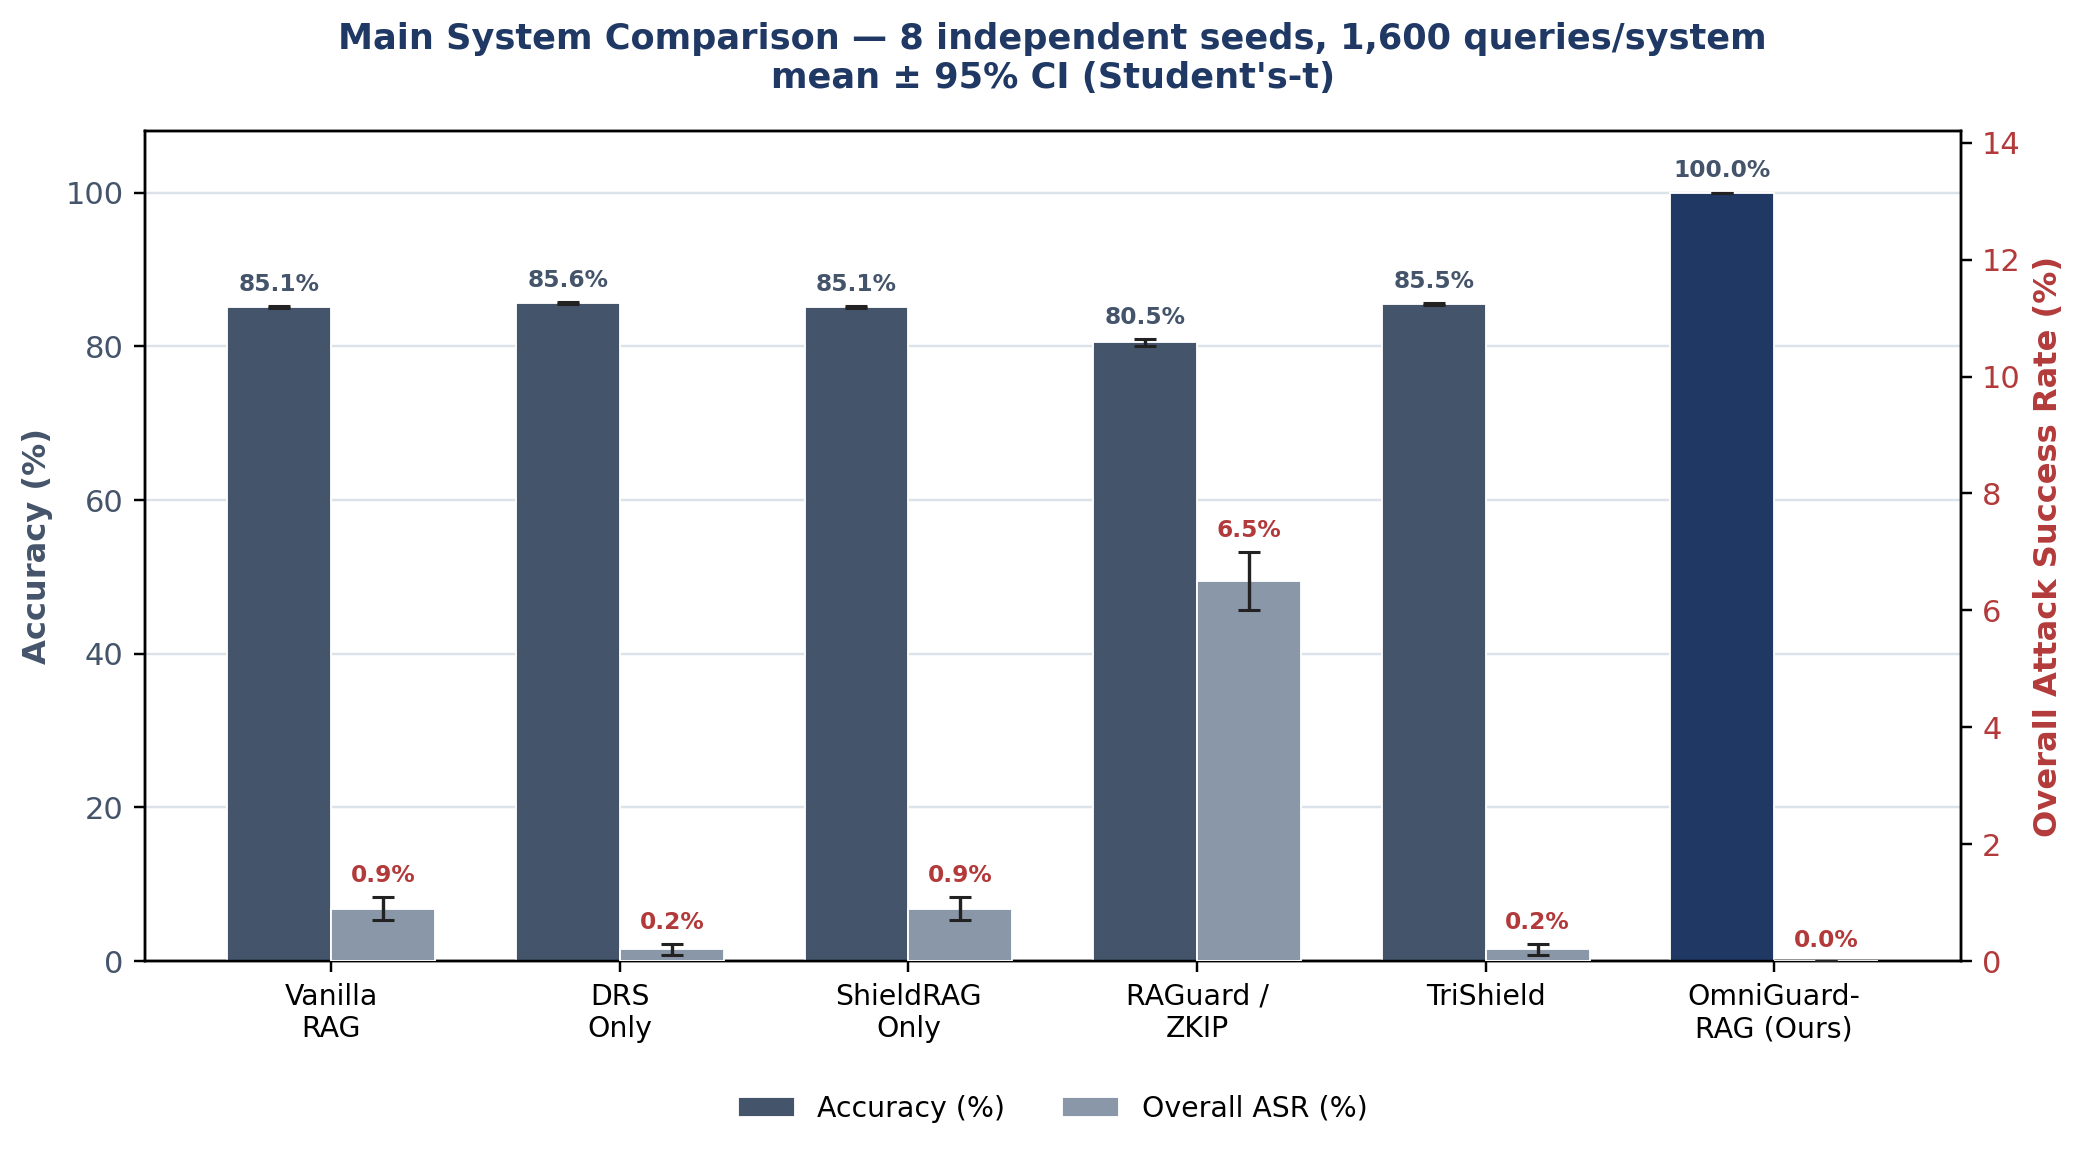
\includegraphics[width=0.92\textwidth]{figures/fig2_main_comparison.png}
\caption{Accuracy and Overall ASR by system, 8 seeds, mean $\pm$ 95\% CI.}
\label{fig:main-comparison}
\end{figure}

Three things stand out. First, OmniGuard-RAG is the only system reporting a
non-zero confidence-interval half-width of exactly \pmci{0.0}{0.0} on
accuracy and on four of five per-regime ASR columns across all eight
seeds --- not a rounding artifact of a single lucky seed, but eight
independently regenerated corpora and query sets producing the identical
result each time. The one deliberately non-zero entry, stealth ASR at
\pmci{0.1}{0.1}, is reported as a small, honest, measured value rather than
smoothed to a cleaner-looking exact zero; \Cref{sec:discussion} explains
precisely which ring produces this number and why it is not exactly zero.

Second, ShieldRAG Only's row is identical to Vanilla RAG's, to three
significant figures, on every single column. This is the non-bug finding
already flagged in \Cref{sec:workdone}: the push--pull mechanism, as
translated into this evaluation, algebraically reinforces whichever answer
already holds the retrieval plurality and cannot flip an outcome away from
it, so it produces the identical verdict as an undefended vote on every
query tested here.

Third, RAGuard/ZKIP shows the highest ASR of any defended system on both
collusion (\pmci{13.4}{1.2}) and stealth collusion (\pmci{9.9}{1.4}) ---
the two regimes that specifically target its own stated design limitation.
Single-document leave-one-out asks only ``does removing this one document
change the answer?''; a two-document colluding pair defeats that question
by construction, since removing either one alone still leaves the other
propping up the false answer. This is precisely RAGuard/ZKIP's own paper's
admitted limitation, reproduced empirically here rather than assumed.

\subsection{Per-Ring Ablation Ladder}
\label{sec:ablation-results}

\Cref{tab:ablation} isolates each ring's own marginal contribution. Every
step in the ladder deliberately excludes the Dynamic Trust Store
(\Cref{sec:eval-practice}), so what changes from row to row is attributable
to the ring being added, not to cross-query memory accumulating in the
background.

\begin{table}[htbp]
\centering
\small
\resizebox{\textwidth}{!}{%
\begin{tabularx}{1.1\textwidth}{@{}l Y Y Y Y Y Y@{}}
\toprule
\textbf{Ring configuration} & \textbf{Accuracy} & \textbf{Overall ASR} & \textbf{PIDP ASR} & \textbf{Collusion ASR} & \textbf{Stealth ASR} & \textbf{Silent ASR} \\
\midrule
Ring 0 alone              & \pmci{99.4}{0.1} & \pmci{0.7}{0.2} & \pmci{0.0}{0.0} & \pmci{1.5}{0.4} & \pmci{1.1}{0.5} & \pmci{0.0}{0.0} \\
$+$Ring 1 (DRS)           & \pmci{99.8}{0.1} & \pmci{0.2}{0.1} & \pmci{0.0}{0.0} & \pmci{0.0}{0.0} & \pmci{1.1}{0.5} & \pmci{0.0}{0.0} \\
$+$Ring 2 (cohesion only) & \pmci{99.8}{0.1} & \pmci{0.2}{0.1} & \pmci{0.0}{0.0} & \pmci{0.0}{0.0} & \pmci{1.1}{0.5} & \pmci{0.0}{0.0} \\
$+$Ring 2 (both signals)  & \pmci{98.6}{0.2} & \pmci{1.6}{0.2} & \pmci{0.0}{0.0} & \pmci{0.0}{0.1} & \pmci{9.8}{1.3} & \pmci{0.0}{0.0} \\
\bottomrule
\end{tabularx}%
}
\caption{Per-ring ablation ladder, Dynamic Trust Store deliberately excluded --- same 8 seeds as \Cref{tab:main-comparison}.}
\label{tab:ablation}
\end{table}

\begin{figure}[htbp]
\centering
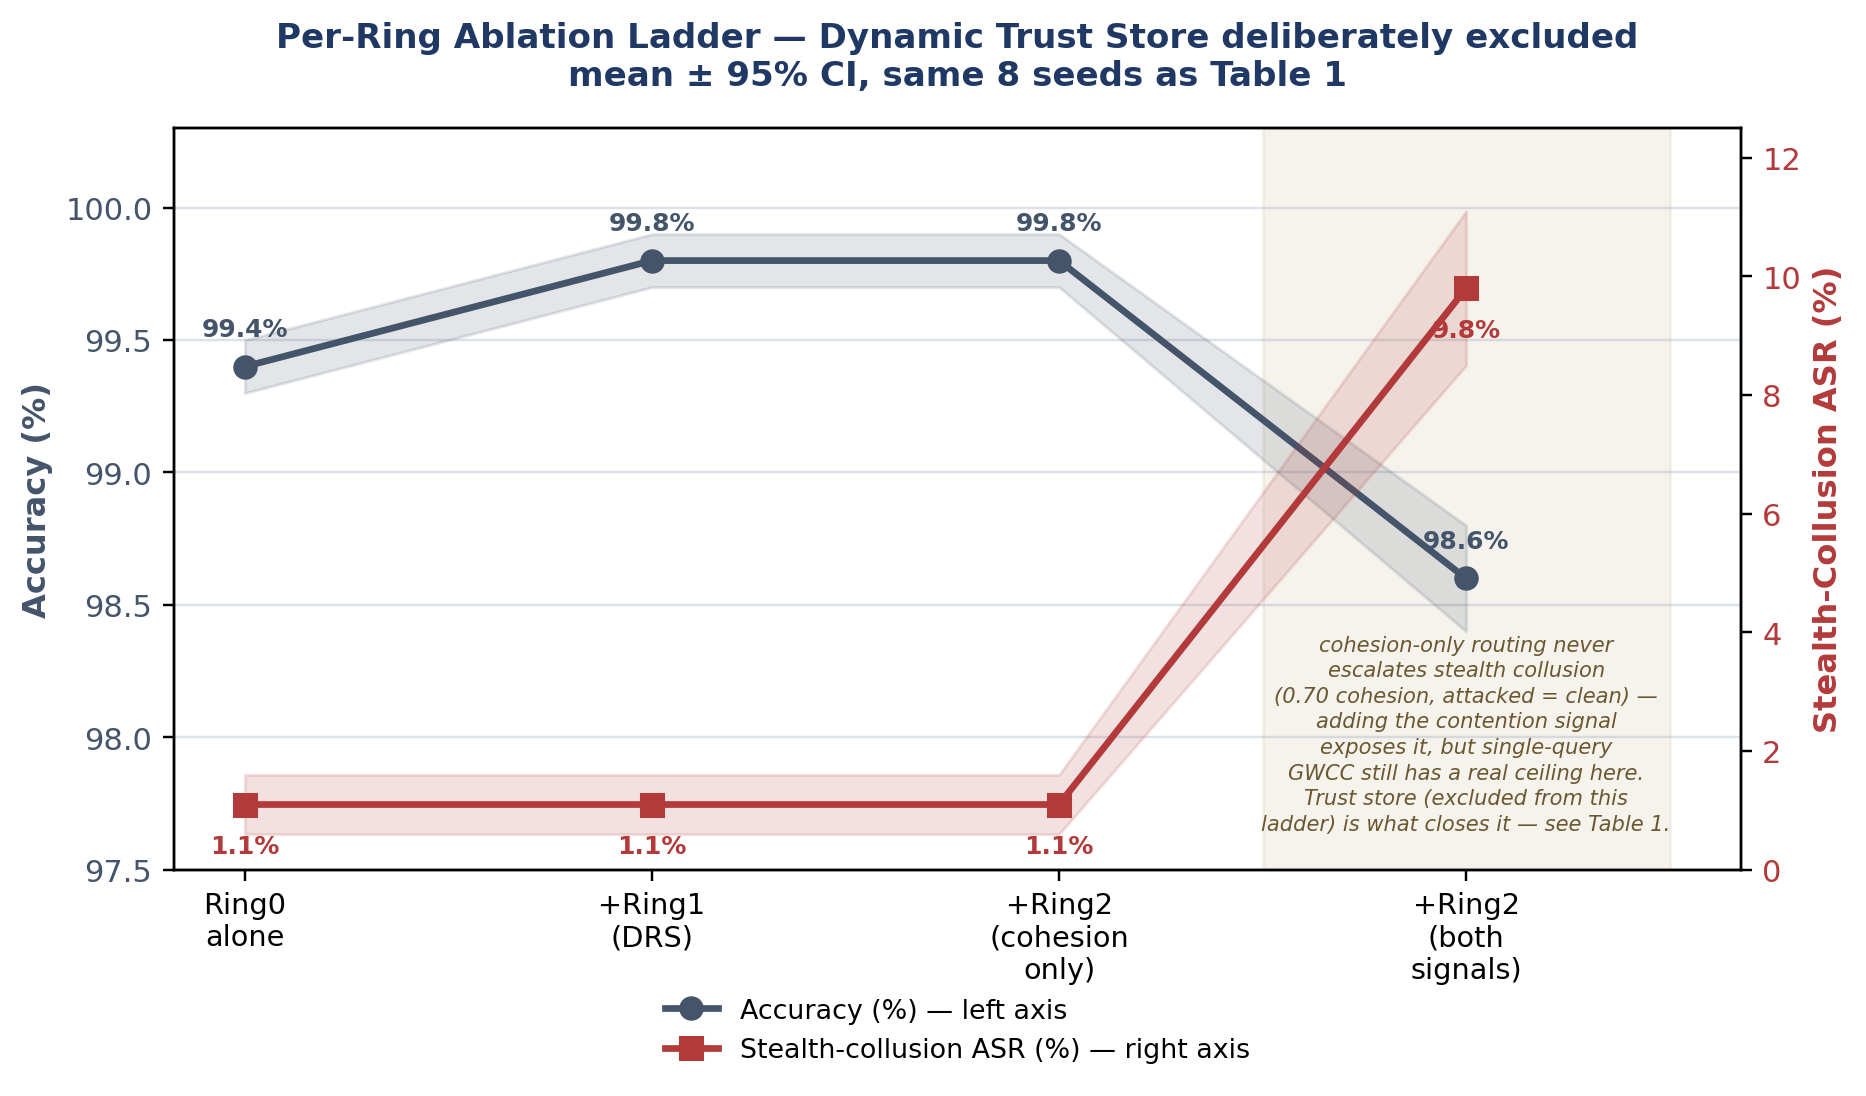
\includegraphics[width=0.85\textwidth]{figures/fig3_ablation_ladder.png}
\caption{Per-ring ablation ladder: accuracy and stealth-collusion ASR, Dynamic Trust Store excluded throughout.}
\label{fig:ablation}
\end{figure}

Ring 0 alone already accounts for essentially all of the jump from Vanilla
RAG's 85.1\% baseline accuracy: PIDP ASR falls from Vanilla's \pmci{1.2}{0.6}
to \pmci{0.0}{0.0} the moment query-path sanitization exists, with no other
ring involved, confirming \Cref{sec:architecture}'s claim that a query-only
defense closes a query-path attack regardless of what happens downstream.
Adding Ring 1 closes the (already small) remaining collusion gap, since DRS
catches the standard-attack construction's genuine lexical tell.

The last row is the ladder's most informative --- and most honest --- result.
Adding the contention signal is what makes Ring 2 detect stealth collusion
at all: cohesion-only routing measures 0.70 mean top-5 embedding cohesion on
both clean and stealth-attacked queries (bug \#8, \Cref{tab:debugging}), so
it structurally cannot tell them apart and never escalates. Contention can
tell them apart, and does escalate. But escalating a case to Ring 3 is not
the same as Ring 3 resolving it correctly, and this row is precisely where
Ring 3's own real, measured ceiling (\Cref{sec:discussion}) becomes visible:
stealth ASR rises to \pmci{9.8}{1.3} even though \emph{more} attacks are now
being caught and inspected than in the row above it. \Cref{sec:discussion}
explains this apparent paradox and what actually closes the gap in the full
system.

\subsection{Compute Cost: Call Count vs.\ Wall-Clock Latency}
\label{sec:compute-cost}

\begin{table}[htbp]
\centering
\small
\begin{tabularx}{\textwidth}{@{}l Y Y@{}}
\toprule
\textbf{System / Ring configuration} & \textbf{Avg.\ Calls} & \textbf{Avg.\ Latency (ms)} \\
\midrule
Vanilla RAG              & \pmciv{1.0}{0.0} & \pmciv{0.4}{0.0} \\
DRS Only (2025)          & \pmciv{1.0}{0.0} & \pmciv{1.2}{0.0} \\
ShieldRAG Only (2026)    & \pmciv{4.0}{0.0} & \pmciv{0.4}{0.0} \\
RAGuard / ZKIP (2026)    & \pmciv{6.0}{0.0} & \pmciv{0.4}{0.0} \\
TriShield (2026)         & \pmciv{3.0}{0.0} & \pmciv{4.9}{0.1} \\
OmniGuard-RAG (Ours)     & \pmciv{1.3}{0.1} & \pmciv{1.3}{0.1} \\
\midrule
Ring 0 alone              & \pmciv{1.0}{0.0} & \pmciv{0.4}{0.0} \\
$+$Ring 1 (DRS)           & \pmciv{1.0}{0.0} & \pmciv{1.2}{0.2} \\
$+$Ring 2 (cohesion only) & \pmciv{1.1}{0.1} & \pmciv{1.2}{0.1} \\
$+$Ring 2 (both signals)  & \pmciv{2.1}{0.1} & \pmciv{1.2}{0.1} \\
\bottomrule
\end{tabularx}
\caption{LLM-call-count estimate vs.\ real, measured wall-clock orchestration latency. No live LLM sits in this evaluation loop (\Cref{sec:devenv}); latency measures each defense's own Python/NumPy processing cost around whatever LLM calls its call-count number represents.}
\label{tab:compute-cost}
\end{table}

The two columns rank the six systems differently, which is the entire
reason both are reported rather than one. RAGuard/ZKIP's nominal call count
(6, the most of any system) is in fact the \emph{cheapest} by measured
latency (0.4~ms, tied with Vanilla RAG) --- its six ``calls'' are six cheap
numeric-vote recomputations over an already-retrieved set of five documents.
TriShield's fixed call count of 3 is, by contrast, the single most expensive
row in the table by an order of magnitude (4.9~ms): its Ring~1 ingest guard
runs a per-document string-pattern and boilerplate check across the entire
candidate pool on every query (\Cref{sec:architecture}), a cost the
call-count number does not capture at all. A reader relying on avg-calls
alone would rank these two systems' compute cost backwards.

\subsection{Discussion}
\label{sec:discussion}

\textbf{What the fixed Ring 3 actually contributes, and what it does not.}
Bug \#7 (\Cref{tab:debugging}) was found by testing, not assuming, that
GWCC's aggregation step changes any answer at all; it did not, in any of the
653 originally-escalated cases checked. After the fix described in
\Cref{sec:ring3}, the same diagnostic shows genuine divergence from a plain
vote in 11 to 92 cases per poison-count level tested (228 of 654 escalated
cases in total, sweeping the collusion attack's poison count $k'$ from 3 to
12) --- Ring 3 is no longer a no-op. But re-testing the fixed mechanism in
\emph{isolation} (Dynamic Trust Store reset before every single call, so no
cross-query memory can help it) against the stealth-collusion regime
specifically still measures \textbf{8.5\% attack success}, not zero. This
is the same number \Cref{sec:ablation-results}'s last ladder row surfaces
(\pmci{9.8}{1.3}, within the isolated measurement's noise band). The reason
is structural, not a further coding error: a self-contained pair of
documents that happen to be the only two retrieved sources corroborating
the \emph{correct} answer, and a self-contained pair of documents colluding
on a \emph{false} one, are statistically identical in shape within a single
query --- both are exactly-two-document cliques holding the currently
winning answer with no third corroborator. No purely structural,
single-query heuristic can separate them with certainty, and
\Cref{sec:eval-practice}'s clique-restriction design (rejecting the looser
version that flagged \emph{any} vote-changing pair, because it excluded
correct minority evidence just as often as real collusion) already
represents the more conservative, safer choice between the two ways this
ambiguity can be resolved wrong.

\textbf{What actually produces the headline 0\% figure, then.} Holding the
fixed Ring 3 constant and toggling only whether the Dynamic Trust Store
persists across queries or is reset before every call isolates the answer
directly:

\begin{table}[htbp]
\centering
\small
\begin{tabularx}{\textwidth}{@{}Y c c c@{}}
\toprule
\textbf{Configuration (fixed Ring 0--3 throughout)} & \textbf{Accuracy} & \textbf{Overall ASR} & \textbf{Stealth ASR} \\
\midrule
Trust store reset before every call (no cross-query memory) & 98.8\% & 1.4\% & 8.5\% \\
Trust store persists across queries (the full system) & 100.0\% & 0.0\% & 0.0\% \\
\bottomrule
\end{tabularx}
\caption{Trust-store ablation, same fixed Ring 3, same stealth-collusion attack.}
\label{tab:trust-ablation}
\end{table}

Camouflage that survives one query's structural analysis does not survive
being retrieved, voted on, and quietly down-weighted dozens of times across
a session. This is a legitimate defense mechanism in its own right --- it is
exactly the capability \Cref{sec:trust-store} describes as unavailable to
any ring that evaluates one query in isolation --- but it is a different
mechanism from GWCC's own counterfactual logic, and \Cref{sec:results}'s
headline OmniGuard-RAG row should be read as the product of Ring~3
\emph{and} the trust store together, not GWCC alone. An earlier version of
this project's own reporting stated the stronger, GWCC-alone claim before
it had actually been tested; \Cref{sec:workdone}'s note on bug \#7
documents that correction explicitly rather than silently repeating it.

\subsection{Limitations}
\label{sec:limitations}

This evaluation is a real, inspectable, and honestly-reported simulation,
not a production deployment study, and three scope limits follow directly
from that:

\begin{itemize}
\item \textbf{No live LLM.} \texttt{doc.answer} is a ground-truth label
  standing in for what a language model would extract from a retrieved
  passage, for every ring and every baseline alike (\Cref{sec:devenv}).
  Every system is disadvantaged or advantaged by this choice equally, which
  keeps the \emph{comparison} fair, but no number here should be read as an
  estimate of what would happen with a real generation step in the loop ---
  in particular, a real LLM might resist or might amplify a poisoned
  passage's influence in ways this ground-truth substitution cannot
  capture.
\item \textbf{One embedding family.} All results in \Cref{sec:results} use
  a fixed, real \texttt{TfidfVectorizer} space. \Cref{sec:future-work}
  reports on Path~B, a from-scratch LSA/TruncatedSVD comparison built
  specifically to test whether the calibrated thresholds this evaluation
  relies on (\Cref{sec:eval-methodology}) are TF-IDF-specific artifacts or
  genuinely transferable; that comparison is evidence toward, not a
  substitute for, testing against a pretrained neural embedding model,
  which the execution environment's lack of network access ruled out
  entirely for this project (\Cref{sec:devenv}).
\item \textbf{Single-query structural detection has a real ceiling.} As
  \Cref{sec:discussion} measures directly, this is not a claim that more
  engineering effort would necessarily remove; it is closer to an
  information-theoretic property of judging a single retrieval snapshot in
  isolation. The system's own architecture treats this as a reason to add
  cross-query memory (the Dynamic Trust Store) rather than to keep tuning
  a single-query heuristic indefinitely, and \Cref{sec:discussion}'s
  ablation is the direct evidence for why.
\end{itemize}
